\documentclass[a4paper]{amsbook} 
\usepackage[T1]{fontenc}
\usepackage[utf8x]{inputenc} 
\usepackage[italian]{babel}

\usepackage{epigraph} 
\setlength{\epigraphwidth}{0.8\textwidth}
\renewcommand{\epigraphsize}{\small}

\usepackage{amsmath}
\usepackage{amsthm} 
\usepackage{amsfonts}
\usepackage{amssymb}

\usepackage[babel=true,final]{microtype} 

%-----------------------
\usepackage{booktabs,enumitem,graphicx,hypernat,xcolor,url}
%\usepackage{booktabs,enumitem,graphicx,hyphenat,titlesec,xcolor,url}
%\usepackage[showframe=false,paper=a4paper,margin=1in]{geometry}
%
\usepackage{hyperref}
%
%\definecolor{titlecolor}{rgb}{0,0,0.5}
%
%\titleformat{\chapter}[display]
%            {\raggedright\normalfont\Large\color{titlecolor}}
%			{\chaptertitlename\ \thechapter}{0pt}{\Huge}[\vspace{5pt}\titlerule]
%\titleformat{\section}
%			{\raggedright\normalfont\Large\bfseries\color{titlecolor}}
%			{\thesection}{1ex}{}
%\titleformat{\subsection}
%			{\raggedright\normalfont\large\bfseries\color{titlecolor}}
%			{\thesubsection}{1ex}{}
%\titleformat{\paragraph}[runin]
%			{\normalfont\normalsize\bfseries}{\theparagraph}{1em}{}
%
%\titlespacing*{\chapter}{0pt}{0pt}{40pt}
%
\usepackage{etoolbox}
%\makeatletter
%\patchcmd{\@dottedtocline}
%  {\rightskip\@tocrmarg}
%  {\rightskip\@tocrmarg plus 4em \hyphenpenalty\@M}
%  {}{}
%\renewcommand{\@pnumwidth}{1.7em}
%\renewcommand{\@tocrmarg}{2.7em}
%\makeatother
%
%
\hypersetup{
	pdftitle={Note per il Corso di Programmazione},
	pdfauthor={Antonio Caruso}}
\hypersetup{
	colorlinks=true,
	linkcolor=black,
	citecolor=black,
	filecolor=black,
	urlcolor=black
}

%\usepackage{boiboites} 

%\newboxedtheorem[
%	boxcolor = red!50!black, 
%	background=blue!5, 
%	titlebackground=blue!20,
%	titleboxcolor=black]{thm}{Teorema}{thmCounter} 
%
%
%\newboxedtheorem[
%	boxcolor = orange, 
%	background=blue!5, 
%	titlebackground=blue!20,
%	titleboxcolor=black]{defn}{Definizione}{defCounter} 
%
%\newboxedtheorem[
%	boxcolor = black, 
%	background=blue!5, 
%	titlebackground=blue!5,
%	titleboxcolor=black]{observe}{Osservazione}{obsCounter} 
%
%%\newboxedtheorem[
%%	boxcolor = black, 
%%	background=blue!2, 
%%	titlebackground=blue!20,
%%	titleboxcolor=black,
%%	size=0.94\textwidth]{ex}{Esempio}{exCounter} 
%

\newtheorem{thm}{Teorema}
\newtheorem{observe}{Osservazione}
\theoremstyle{definition}
\newtheorem{ex}{Esempio}

%\usepackage{setspace} 
%\setstretch{1.02} 
\setlength{\parskip}{0.1em}

%% ------------------- Front matter ------------------------ 
%
\makeatletter
\renewcommand\maketitle{
\begin{titlepage} \vspace*{\stretch{1}}
\begin{center} {\Huge \@title \par}%
	 \vspace{5em}%
	 {\LARGE Antonio Caruso \par}%
	 \vspace{1.5em} {
	 \large \emph{\@date} \par}%
	 \vspace{3em} \end{center}%
\vspace*{\stretch{1}}
\end{titlepage}}
\makeatother

\clubpenalty=10000 
\widowpenalty=10000 
\overfullrule=1mm

\newcommand{\nota}[1]{\marginpar[{\raggedleft\small\sffamily #1\\}]{%
 								 {\raggedright\small\sffamily #1\\}}}
\newcommand{\Mod}[1]{\ \text{mod}\ #1}


\hyphenation{rap-pre-sen-ta-zio-ne}

\includeonly{chapters}

\setcounter{secnumdepth}{3}
\setcounter{tocdepth}{2}

%% ------------------- Document ------------------------
\begin{document}

\frontmatter 
\title{Note per il Corso di Programmazione}
\author{Antonio Caruso} 
\address{\centering
 Dipartimento di Matematica e Fisica 'Ennio De Giorgi'\newline
 \centering Complesso Ecotekne, Palazzo Fiorini
}
\email{antonio.caruso@unisalento.it}
\date{a.a. 2015/16}
\begin{abstract}
	Queste Note sono parte del materiale didattico per il corso di Programmazione, della Laurea Triennale in Matematica.
\end{abstract}
\maketitle
\addtocontents{toc}{~\hfill\textbf{Page}\par}
\tableofcontents
\mainmatter

\pagenumbering{arabic}
\pagestyle{headings}

%\newgeometry{vmargin=30mm, right=1.9in, marginparsep=3.5mm, footskip=15mm}
%\hypersetup{pageanchor=true} 

%!TEX root = note.tex

\chapter{Rappresentazione dei Numeri}

\epigraph{I do hate sums!! There is no greater mistake than to call arithmetic
an exact science. There are $\ldots$ hidden laws of Number which it requires a
mind like mine to perceive. For instance, if you add a sum from the bottom up,
and then again from the top down, the result is always different!}{ -
\textsc{M. P. LA TOUCHE} (1878)}

\epigraph{Vedete, non esiste nulla (amati studenti in Matematica) che sia così
fastidioso nella pratica matematica, e più molesto che dover calcolare
moltiplicazioni, divisioni, e radici quadrate o cubiche di numeri molto grandi.
A parte la noia e lo spreco di tempo, queste sono spesso soggette a errori
scivolosi. Ho cominciato a considerare nella mia mente, con quale arte io possa
rimuovere tali ostacoli.} { - \textsc{JOHN NEPAIR [Napier] (1916)}}

\section[Numeri Interi]{Numeri Interi}

Il primo approccio con la Matematica è \emph{contare}. Il contare porta alla
definizione dei numeri interi, attualmente scritti attraverso l'uso di una
\emph{notazione posizionale decimale} che come vedremo è stata introdotta in
Europa intorno al A.D. $1202$\footnote{Quindi per migliaia di anni il modo con
cui si pensava ad i numeri, li si scriveva e sopratutto si faceva Aritmetica è
stato molto diverso da come noi siamo abituati a fare sin da piccoli.} da parte
di Leonardo Pisano (detto il Fibonacci). Gli Interi e le operazioni elementari
tra essi, come somma, sottrazione, moltiplicazione e divisione sono studiati in
quella parte della matematica chiamata \emph{Aritmetica}; Nonostante il lettore
possa trovare strano dover rivedere concetti che ritiene assodati, vedremo come
l'Aritmetica meriti senz'altro un ulteriore approfondimento.

Queste note introdurranno una diversa prospettiva sul perché scriviamo i numeri
in decimale. Vedremo come la scelta di una rappresentazione numerica è
strettamente legata al modo con cui svolgiamo abitualmente le operazioni
aritmetiche, cioè gli \emph{algoritmi} usati per il calcolo di somma,
sottrazione, etc. Questi aspetti sono di interesse sia per comprendere
all'interno del corso di Programmazione come viene rappresentata l'informazione
dentro il computer, sia per chi dovrà svolgere attività didattica nelle scuole
elementari; evidenziando la natura essenzialmente \emph{algoritmica}
dell'Aritmetica.

Siamo interessati in particolare allo studio della \emph{rappresentazione} dei
numeri. In questa prospettiva dobbiamo chiaramente sottolineare la differenza
tra due entità: un numero, inteso astrattamente come \emph{valore} e la sua
\emph{rappresentazione} (o \emph{numerale}) intesa come sequenza di segni che
servono appunto a scrivere o comunicare un certo valore. Cominciamo quindi,
\nota{rappresentazione vs.\\ valore} con il distinguere chiaramente un valore
numerico, ad esempio l'intero $1234$, da una delle sue tante possibili
\emph{rappresentazioni}, termine che vuol indicare \emph{il modo in cui
scriviamo} quel valore. Noi scriviamo (e pensiamo) i numeri allo stesso modo,
usando un sistema posizionale \emph{decimale} pertanto il modo più comune di
scrivere $1234$ è ovviamente: \textsf{'1234'}\footnote{le due scritture sono
diverse per enfatizzare che $1234$ è il valore, ed \textsf{'1234'} solo un modo
particolare per scrivere tale valore.}, ma lo stesso numero sarebbe stato
scritto come \textsf{'MCCXXXIV'} se vivessimo nell'antica Roma. Una
rappresentazione numerica è una serie di convenzioni più o meno formalizzabili
che descrivono come si \emph{scrivono} i numeri, cioè una serie di regole
\emph{'sintattiche'} che possono variare nel tempo e nello spazio.

La rappresentazione posizionale, ci consente di scrivere qualunque numero
(naturale) come una \emph{stringa}\footnote{sequenza di caratteri giustapposti}
di \emph{cifre} (\emph{digit} in inglese). Vale il seguente Teorema:


%%% Definizione Rappresentazione Posizionale


\begin{thm}[Rappresentazione dei numeri Naturali in base $B$] Sia $B>1$ un
intero che chiameremo \emph{base (o radice)} della rap\-presentazione, e
$\mathcal{C} = \{ c_0, c_1, \ldots c_{B-1} \}$ un insieme di simboli distinti
dette \emph{cifre della rappresentazione} (in inglese \emph{digit}). Ogni cifra
è associata ad un valore intero tra $0$ e $B-1$.\bigskip

Allora $\forall n \in \mathbb{N}$, esiste ed è unica la sequenza di cifre:
$(c_{k-1}c_{k-2} \ldots c_1c_0)_B$ ed il suo valore è:
\begin{equation}\label{eq:pos} 
n = c_{k-1}B^{k-1}+c_{k-2}B^{k-2}+\ldots+c_1B+c_0 = \sum_{i=0}^{k-1} c_iB^i
\end{equation} \end{thm} %%%%

Il sistema \emph{decimale} ha $B = 10$ e $\mathcal{C} = $\{\textsf{ 0, 1, 2, 3,
4, 5, 6, 7, 8, 9}\,\} ed il lettore lo usa quotidianamente fin dalle
elementari. \nota{sistema decimale, binario, ternario,.. esadecimale} Con $B =
2$ come vedremo il sistema è detto binario e lo tratteremo approfonditamente,
con B = 3 abbiamo numeri in ternario, con $B = 4$ in quaternario, con $B = 8$
in ottale. Possiamo avere anche $B > 10$, ad esempio con $B = 16$ abbiamo il
sistema esadecimale, le cifre comunemente usate nel sistema decimale non
bastano a rappresentare i simboli delle cifre esadecimali, e si usa normalmente
$\mathcal{C} = \{ \textsf{0,1,2,3,4,5,6,7,8,9,A,B,C,D,E,F} \}$ con la
convenzione che $\textsf{A} = 10, \textsf{B} = 11, \ldots, \textsf{F} = 15$.

\begin{ex} $(\textsf{1234})_{10} = 1\cdot 10^3+2\cdot 10^2 + 3 \cdot 10 + 4 =
1234$. $(\textsf{1234})_8 = 1\cdot 8^3+2\cdot 8^2+3\cdot 8^1+4\cdot 8^0 =
(668)_{10}$. $(\textsf{11010010})_2 = 1\cdot 2^8 + 1\cdot 2^7 + 1\cdot 2^5 +
1\cdot 2^1 = (1234)_{10}$. $(\textsf{1ABF})_{16} = 1\cdot 16^3 + 10\cdot 16^2 +
11 \cdot 16 + 15 = 6848_{10}$. $(\textsf{4D2})_{16} = 4\cdot 16^2 + 13\cdot 16
+ 2 = 1234_{10}$.

\noindent $(\textsf{1234})_3$ ? La sequenza non rispetta le condizioni del
Teorema, non ha quindi molto senso valutarla poiché se $B = 3$ si ha
$\mathcal{C} = \{ 0, 1, 2 \}$ ed i simboli \textsf{3,4} non hanno alcun
significato in tale sistema. \end{ex}

Nel seguito se la base $B$ è chiara dal contesto non useremo le parentesi e la
base come pedice, pertanto $ (1001001)_2$ sarà scritto semplicemente come
$1001001$ se è chiaro che stiamo trattando numeri in base $2$. Noi usiamo
abitualmente la base $10$ per cui scriviamo abitualmente \textsf{1298} e non
$\mbox{\textsf{(1298)}}_{10}$, ed il valore ad esso associato è l'intero 1298.
Quest'ultima osservazione che può sembrare banale è invece opportuna in quanto
è chiaro che data una sequenza di cifre, il valore ad essa associato dipende
dal sistema di numerazione in cui ci troviamo, cioè dalla base usata, la stessa
sequenza infatti avrà valori diversi per basi diverse.

La condizione $0 \leq c_i \leq B-1$\nota{Condizione per l'esistenza e unicità
della rappresentazione} è essenziale per garantire l'esistenza e l'unicità
della rappresentazione. Nell'Esempio precedente abbiamo scritto che non ha
senso valutare $(1234)_3$, proviamo ad essere più precisi: consideriamo $B = 2$
e supponiamo vi siano $4$ cifre: $\mathcal{C} = \{ 0, 1, 2, 3 \}$ vediamo
subito che l'unicità della rappresentazione non vale più poiché $13 = 3\cdot
2^2 + 1 \cdot 2^0$ ma anche $2\cdot 2^2 + 2\cdot 2^1 + 1\cdot 2^0$. Quindi se
usiamo \emph{troppe} cifre, perdiamo l'unicità, allo stesso modo se usiamo
\emph{poche} cifre perdiamo l'esistenza di una rappresentazione, ad esempio se
in base $10$ usassimo solo le cifre $0,\ldots,8$ avremmo infiniti numeri
naturali non rappresentabili ($9$, $19$,..).

Il valore $k$ in \eqref{eq:pos} è il numero di cifre, le singole cifre prese da
$\mathcal{C}$ hanno significato diverso in base alla loro posizione, ecco
perché il sistema è detto posizionale. Il peso è proporzionale ad una potenza
della base via via crescente da destra a sinistra. La prima cifra $c_{k-1} \neq
0$ viene detta \emph{più significativa} poiché associata alla potenza della
base più alta, corrispondentemente la cifra $c_0$ o cifra delle \emph{unità}
viene chiamata anche \emph{meno significativa}. Vale la pena ricordare che
nella didattica della Matematica nelle classi primarie (elementari) è usuale
dare dei numeri come $1214$ e chiedere di scomporli nelle loro cifre e nei pesi
della base attraverso la dizione seguente:

{\it 1214 $ = $ un migliaio, due centinaia, una decina, e quattro unità.}

\noindent in questo modo i bambini apprendono rapidamente che le cifre
rappresentano valori differenti a secondo della loro posizione, e che tale
valore è proporzionale ad un opportuna potenza della base (a questo livello
identificate con opportune espressioni: migliaia, centinaia, etc). Dimostriamo
adesso il Teorema:

\begin{proof}%[(Teorema 1)]
Fissiamo la base $B$ e dimostriamo esistenza e unicità di \eqref{eq:pos} per induzione su $n$.

Chiaramente $1$ è sempre rappresentabile in uno ed un solo modo\footnotemark. Adesso supponiamo induttivamente che ogni intero
$1,\ldots,n-1$ sia rappresentabile in modo univoco.

\noindent Consideriamo l'intero $n$, chiamiamo $d = n \mod B$, allora $d < B$ è una delle cifre disponibili. Per induzione $n' = (n-d)/B$ è unicamente rappresentabile, diciamo ad esempio così:
\[ \frac{n-d}{B} = d_0 + d_1 B + d_2 B^2 + \ldots \]
Allora chiaramente
\begin{align*}
n = d + \frac{n-d}{B}B = d + d_0 B + d_1 B^2 + d_2 B^3 + \ldots
\end{align*}
è una rappresentazione di $n$ che usa solo le cifre disponibili, e l'esistenza è dimostrata.
Adesso supponiamo che $n$ abbia due rappresentazioni diverse avremmo:
\begin{align*}
n &= a_0 + a_1B + a_2B^2 + \cdots\\
  &= c_0 + c_1B + c_2B^2 + \cdots
\end{align*}
Ma poichè da sopra, $c_0$ e $a_0$ sono uguali a $d = n \mod B$, allora sono eguali, quindi la differenza deve essere nelle altre cifre. Ma allora il numero $n'$ ha due rappresentazioni diverse, ma questo
contraddice l'ipotesi induttiva.
\end{proof}\footnotetext{perche?}

Svolgendo le operazioni in \eqref{eq:pos} in base $10$ abbiamo un modo semplice
per convertire un naturale dalla base $B \neq 10$ alla base $B = 10$.
Nell'esempio precedente mostriamo come convertire numeri binari, ottali o
esadecimali in decimale. La stessa formula ci mostra come i numeri siano
strettamente collegati al concetto di polinomio: la somma in \eqref{eq:pos} può
essere vista come un polinomio di grado $k-1$, i cui coefficienti sono le cifre
dell'intero, valutato nel punto $x = B$.

In seguito tratteremo in modo approfondito l'uso della base due\nota{Sistema
Binario}. Se consideriamo $B = 2$ e $\mathcal{C} = \{ 0, 1 \}$ il sistema è
chiamato \emph{binario} proprio perché le cifre a disposizione sono solo due.
Le singole cifre vengono anche chiamate $\emph{bit}$ dalla contrazione di
\emph{Binary digIT}\nota{Bit} (che non è altro che l'inglese di "Cifra
Binaria").

E' nozione\nota{Sistema Binario, Circuiti Bistabili, Hardware
del Calcolatore} comune che le informazioni all'interno di un calcolatore digitale
sono rappresentate in binario, ovviamente come \emph{lunghe} sequenze di bit.
Questo rende tale sistema importante per la comprensione di come viene
codificata l'informazione dentro un calcolatore. L'uso della base due è
motivato dal fatto che è molto semplice misurare una piccola variazione di
potenziale in un circuito, e definire così due \emph{stati} distinti: possiamo ad
esempio associare a $0V$ (Volt) il valore $0$ ed $1$ al livello $+3V$. Se un
circuito può assumere in modo stabile due livelli (non necessariamente quelli
indicati sopra), è detto \emph{bistabile} e consente di rappresentare una cifra
binaria. La procedura con cui convertiamo l'informazione in sequenze di bit
viene detta comunemente \emph{digitalizzazione}. In informatica il termine bit,
indicherà quindi una cifra ($0/1$) di un numero binario, ma in alcuni contesti
si indicherà con lo stesso termine il circuito bistabile usato per memorizzare
un bit.

Osserviamo subito alcune proprietà dei sistemi posizionali:

Se \emph{fissiamo} il numero di cifre ad un massimo di $k$ il numero di valori
che possiamo rappresentare è chiaramente limitato. Il minimo è ovviamente $0$
(se $\forall i \, c_i = 0$). Il massimo si ha quando ogni \nota{Interi in base
$B$ con massimo $k$ cifre:\\ Range = $[0,B^k-1]$} cifra assume il valore
massimo, cioè se $\forall i\, c_i = B-1$ quindi:

\begin{observe} Con $k$ cifre in base $B$ dalla \eqref{eq:pos} si ha:
\begin{equation}\label{eq:range} \sum_{i=0}^{k-1} (B-1)B^i = (B-1)
\sum_{i=0}^{k-1} B^i = (B-1) \frac{1-B^k}{1-B} = B^k-1 \end{equation} Ed i
numeri rappresentabili sono gli interi nell'intervallo $[0,B^k-1]$.
\end{observe}

\noindent dove la penultima equivalenza deriva dalla somma finita (con indici
generalizzati) di una serie geometrica, i.e. per $a,b \in \mathbb{N}$, si ha:
\[ \sum_{i=a}^{b} x^i = \frac{x^a-x^{b+1}}{1-x\quad} \]

Un altro modo \nota{Isomorfismo tra numeri di al più $k$ cifre e $k$-tuple} per
ottenere \eqref{eq:range} senza molti conti è il seguente: invece di scrivere
le cifre tramite una sequenza di caratteri (una stringa) possiamo scriverle
ognuna come componente di una $k$-tupla\footnote{Una $k$-tupla è una
generalizzazione del concetto di coppia, tripla, quadrupla..con $k$ componenti.
In generale è un elemento del prodotto cartesiano di $k$ insiemi.}, quindi la
rappresentazione in \eqref{eq:pos} diventa $(c_{k-1}, c_{k-2}, \ldots,
c_0)$\footnote{La presenza delle virgole non è una differenza da poco: in
\eqref{eq:pos} usiamo una stringa di cifre. i.e. le cifre sono
\emph{giustapposte} senza separatori, in una tupla le componenti sono
chiaramente separate dalle virgole. Le due rappresentazioni sono
matematicamente diverse anche se ovviamente isomorfe.} allora ogni numero con
$k$ cifre può essere visto come un elemento di $\mathcal{C}^k$ (il prodotto
cartesiano di $\mathcal{C}$ per se stesso, $k$ volte), ma la cardinalità di
quest'ultimo insieme è banalmente $|\mathcal{C}^k| = |\mathcal{C}|^k = B^k$,
quindi vi sono $B^k$ configurazioni diverse ed ognuna rappresenterà un intero
diverso; Poichè iniziamo a contare da $0$ il valore massimo rappresentabile
sarà $B^k-1$.

\begin{ex} In base 10 con 4 cifre abbiamo i valori da $0$ a $9999$, cioè
l'insieme $\mathcal{C}^4 = \left\{ (c_3,c_2,c_1,c_0) \;|\; 0 \leq c_i \leq 9
\right\}$ $= \{ (0,0,0,0),$ $\ldots, (9,9,9,9) \}$. Vi sono quindi
$|\mathcal{C}^4| = 10^4 = 10000$ numeri possibili, da $0$ a $9999 =
10^4-1$.\medskip

Se usiamo la base $B = 2$ i valori possibili vanno da $0$ a $1111 =
2^3+2^2+2^1+2^0 = 2^4-1 = 15$, con $8$ bit abbiamo $2^8 = 256$ valori, tra $0$
e $(11111111)_2 = 255$. In esadecimale con $4$ cifre abbiamo $16^4 = 65536$ valori possibili, da $0$ a $\text{FFFF} = 65535$.
\end{ex}

L'esempio\nota{Il numero di cifre per $n$ è $k = \lceil\, \log_B{n} \,\rceil$}
mostra quindi che se fissiamo il numero di cifre, l'intervallo di
rappresentazione aumenta all'aumentare della base. Quante cifre servono a
rappresentare un generico intero? Se $n \in \mathbb{N}$, il numero di cifre
necessario a rappresentare $n$ sarà ovviamente il minimo $k$ tale che $B^k-1
\geq n$, quindi $k = \log_B{n+1} \;\approx\; \lceil\, \log_B{n} \,\rceil$.

\begin{ex}[Numero di cifre di un intero in base $B$] L'ultima relazione ci dice
che la lunghezza in cifre di un numero intero $n$ in decimale è
$\lceil\log_{10} n \rceil$, il che è un ovvia conseguenza della \eqref{eq:pos}.
Prendiamo $n = 123456789$, esso ha $\lceil \log_{10} n \rceil = \lceil\, 8,0915
\,\rceil = 9$ cifre, poiché $\log_2{n} = 8,0915 / \log_{10}{2} = 26,87$, in
binario serviranno $27$ bit. Infatti come vedremo successivamente: $123456789 =
(111010110111100110100010101)_2$. \end{ex}


\subsection*{Lo Zero, l'Unario, i Numeri Romani}
{ \small
Perche usiamo la notazione posizionale, ed in particolare il sistema decimale?
E come sono stati rappresentati i numeri interi prima della diffusione del
sistema decimale?

Sappiamo che in passato alcune popolazioni hanno usato in ambiti specifici
numeri in base $60$ o in base $12$, ma è evidente che la preferenza per il
sistema decimale sia attribuibile alla presenza di dieci dita, che ha reso
molto naturale il suo apprendimento. Resta da capire perché preferire un
sistema posizionale rispetto ad esempio a quello romano?

Cominciamo a rispondere alla domanda precedente, rivedendo come sono stati
scritti o meglio 'segnati' i numeri fin dagli albori del tempo. Il modo
primitivo per rappresentare delle quantità intere è stato l'uso di pietre
(\emph{calculi}) che rappresentavano le unità, dallo stesso termine deriva
l'etimologia di \emph{calcolare}.

Dal punto di vista astratto possiamo vedere questo modo di rappresentare i
numeri come quello di un uomo che chiuso in una cella segna i giorni con delle
tacche su un muro. Questo sistema usa un solo simbolo '\textsc{I}' per
rappresentare le unità, può rappresentare un qualunque numero intero
semplicemente \emph{giustapponendo} un pari numero di simboli, quindi 2 =
\textsc{II}, 3 = \textsc{III}, 4 = \textsc{IIII}, 5 = \textsc{IIIII}, etc.
Questo sistema viene chiamato \emph{unario}.\nota{Sistema Unario} Per quanto
esso sia estremamente semplice, anche per svolgere le operazioni
aritmetiche\footnote{Il lettore provi a definire in modo chiaro, come svolgere
le operazioni aritmetiche in unario.}, esso è affetto da un problema
fondamentale: la lunghezza dei numeri cresce \emph{esattamente} come il numero
da rappresentare: ci vogliono $n$ 'I' per rappresentare $n$. Questo rende
impraticabile la rappresentazione di numeri anche relativamente piccoli, (il
lettore provi a immaginare di scrivere in unario $53$). Nei sistemi posizionali
la rappresentazione è esponenzialmente più corta, in quanto il numero di cifre
come abbiamo visto è solo $\log n$ (Per cinquantatre bastano due cifre), e
questa differenza è forte anche rispetto al più semplice sistema posizionale,
quello binario, che tra tutti è quello che richiede più cifre.

Assodata la difficoltà di utilizzo di un sistema unario, l'unico modo per
migliorare le cose è quello di aumentare il numero di simboli. Ma a questo
punto dobbiamo stabilire che valore dare a diversi simboli, e in quali
circostanze.

I Romani\nota{Numerazione\\ Romana} hanno sviluppato un sistema a
\emph{sostituzione} in cui ogni volta che la rappresentazione di un valore
diventa troppo lunga, si associa tale valore ad un diverso simbolo: poiché $5 =
\mathrm{IIIII}$ è già troppo lungo, introduciamo $\mathrm{V} = 5$, ed essendo
quattro, uno prima di cinque, abbiamo $4 = \mathrm{IV}$, naturalmente $6$ è uno
dopo $5$ quindi $\mathrm{VI}$ e con lo stesso identico sistema possiamo
introdurre $\mathrm{X} = 10, \mathrm{L} = 50, \mathrm{C} = 100, \mathrm{D} =
500, \mathrm{M} = 1000$ e rappresentare $2015 = \mathrm{MMXV}$ con solo quattro
cifre (notare l'assenza dello zero). Il sistema consente di scrivere numeri
senza l'esplosione esponenziale della loro lunghezza come nell'unario, ma è
comunque affetto da numerosi problemi.

\begin{wrapfigure}[10]{r}{4.5cm}
\vspace{-2ex}
\captionsetup{font=small}
\centering 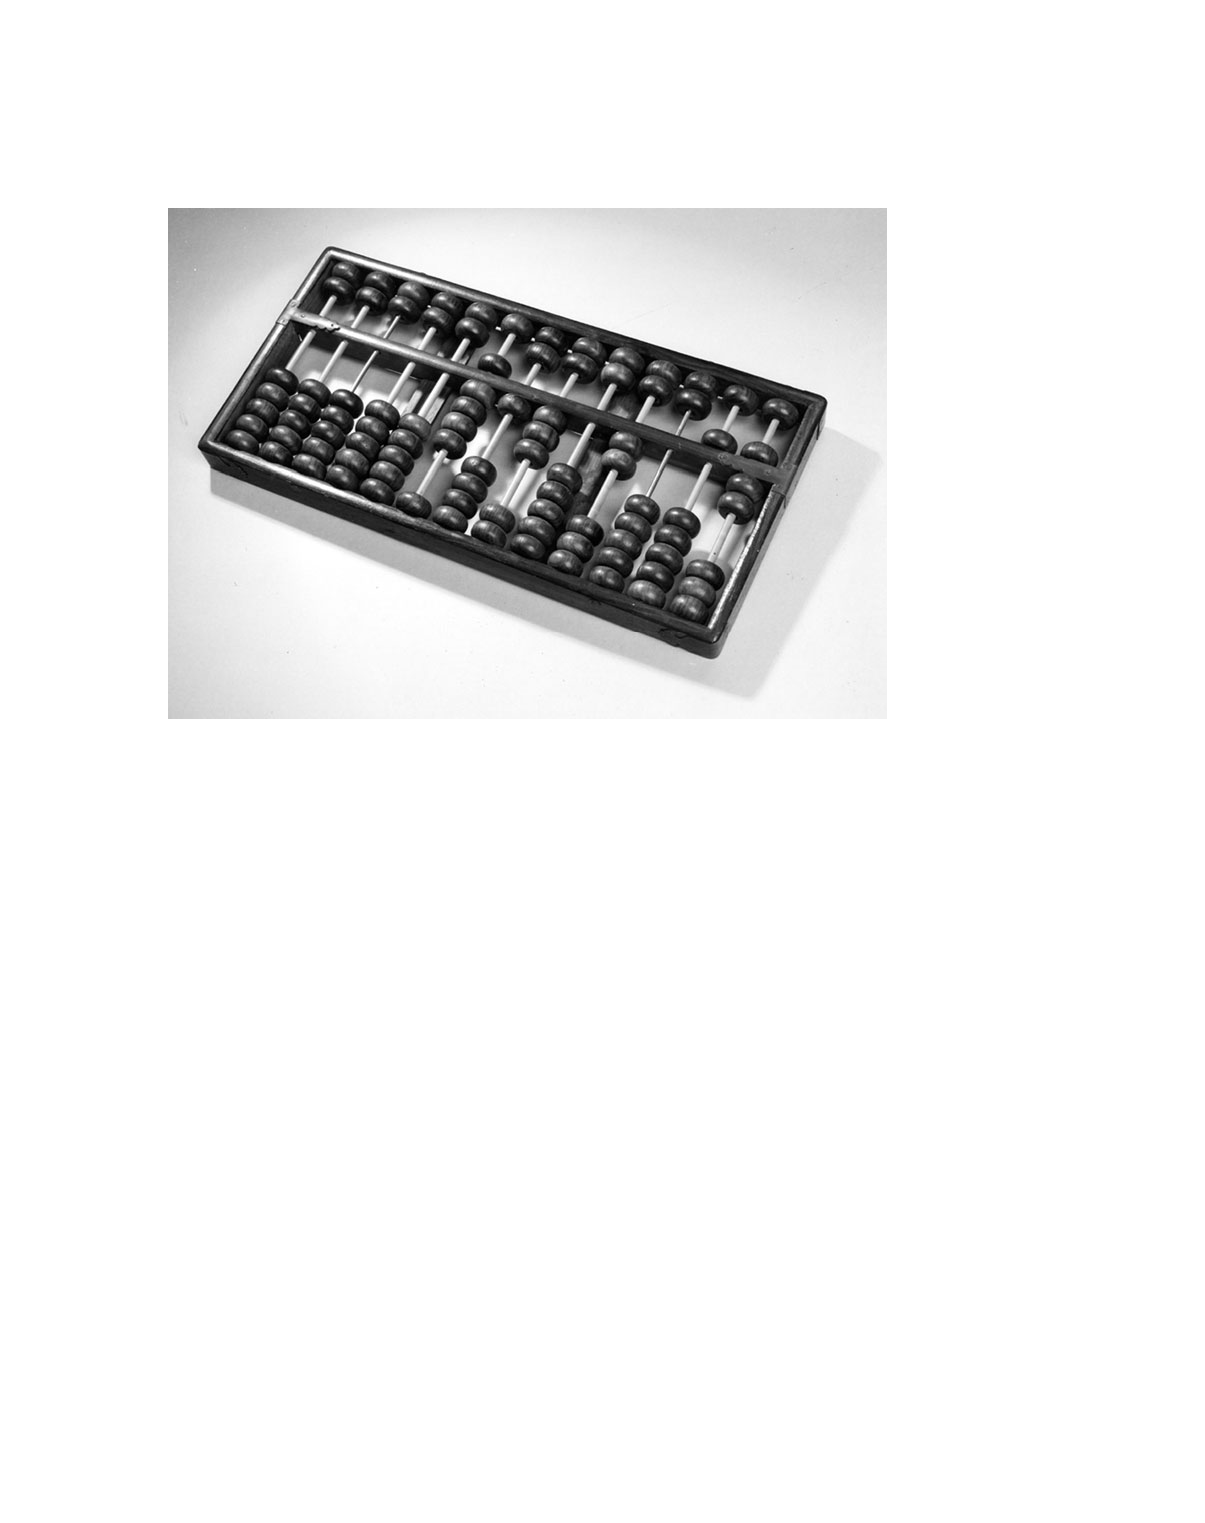
\includegraphics[width=4cm]{abaco.pdf}
\caption{Abaco}\label{fig:abaco}
\end{wrapfigure}
Il numero di simboli non può essere costante come nei sistemi posizionali, ma
deve crescere, cosa accadrebbe se vogliamo rappresentare $10^9$ in romano?
servono altri simboli dopo $\mathrm{M}$. Più importante ancora è la difficoltà
dell'aritmetica: Come possiamo descrivere le operazioni di somma o sottrazione?
In effetti tali operazioni non sono per nulla facili da descrivere, e
sicuramente sono decisamente più complesse rispetto all'aritmetica decimale. I
romani in pratica usavano fare le somme usando un \emph{abaco} (vedi Figura \ref{fig:abaco} accanto) 
solo per numeri molto piccoli.

Gli storici della matematica credono che l'uso della notazione posizionale decimale e l'introduzione dello \emph{zero} siano da attribuire a \emph{Brahmagupta} un matematico indiano nel 620\textrm{AD}. Questo sistema raggiunge l'Europa passando prima attraverso la Spagna (allora Musulmana) e diffondendosi in Italia. L'italiano Leonardo di Pisa, chiamato anche il Fibonacci, scopre questo sistema di numerazione e l'aritmetica ad esso associata lavorando nella bottega del padre, nella città di Bugia (una città Africana nella regione corrispondente all'attuale Algeria).
E' attraverso gli scritti di Muhammad ibn Musa al-Khwarizmi, Abu Kamil e altri\nota{Muhammad ibn Musa al-Khwarizmi} matematici arabi che Fibonacci apprende il nuovo sistema, e lo diffonde in Europa dove viene presto adottato insieme all'uso dello zero. 

E' evidente\nota{Zero in\\ Matematica} l'importanza sia pratica (all'interno
del sistema di numerazione) sia concettuale dello zero. Il fatto che dovesse
esistere un \emph{numero} che indicasse un \emph{assenza} di quantità, è un
concetto che richiese secoli prima di essere assimilato. Lo zero è fondamentale
all'interno dei sistemi posizionali, lo studente oramai capisce la motivazione
di fondo: in un intero come $5005$, gli zeri sono essenziali per \emph{spostare
il peso di una cifra senza aggiungerne complessivamente al valore} (vedi i due
$5$). Una volta introdotto è necessario capire come le operazioni aritmetiche
si comportano su esso, e naturalmente si nota subito il problema legato alla
divisione. Il fatto che l'operazione di divisione \emph{non fosse definita}
(oggi diremmo che essa costituisce una funzione parziale sugli interi) è
qualcosa che contrariava molti matematici. Non parliamo delle resistenze dei
filosofi a dare un nome a una quantità per rappresentare....un assenza di
quantità.
}

\subsection{Conversione tra basi}\label{sec:conversione}

Di seguito si vedrà come convertire da una rappresentazione in base $b$ ad una
in base $B$. Poiché noi siamo abituati a svolgere operazioni in base $10$, per
facilitare il cambio di base, trasformeremo prima un valore dalla base $b$ di
partenza alla base $10$, e poi convertiremo il valore decimale ottenuto in base
$B$. Come visto anche nell'esempio $1$, la formula in \eqref{eq:pos} ci
consente di convertire un numero da una base qualunque alla base $10$. Pertanto
resta da capire come convertire da base $10$ ad un altra base generica $B$.
Osserviamo che dato un intero $n$, l'essenza della dimostrazione del Teorema
$1$ è la riscrittura dell'equazione \eqref{eq:pos} come\footnote{Questo è un
altro esempio del parallelismo tra numeri e polinomi, infatti questo modo di
scrivere i polinomi è detto formula di Horner ed è molto usata per velocizzare
la valutazione del polinomio in un punto.}:

\begin{align*}
n = \sum_{i=0}^{k-1} c_iB^i = (((c_{k-1}B+c_{k-2})B\ldots+ c_2)B + c_1)B + c_0\\
\text{i.e. } 1234 = ((1\cdot{10}+2)\cdot{10}+3)\cdot{10} + 4
\end{align*}


\noindent quindi la cifra meno significativa $c_0$ può essere ottenuta
dividendo (usiamo la divisione intera) $n$ per $B$ e prendendo il resto.
\nota{Conversione in base B, tramite divisioni ripetute per~B ed estrazione dei
resti.} Quindi abbiamo $c_0 = n \Mod{B}$ ed il valore della divisione $n' = n /
B$ è un intero formato dalle rimanenti cifre di $n$. Possiamo ripetere il
procedimento su $n'$ fin quando il valore della divisione è diverso da zero estraendo così tutte le cifre.

\begin{ex}
Consideriamo $n = 12345$, abbiamo $n' = n/10 = 1234$ e $n \Mod{10} = 5$. Ripetendo l'operazione di modulo su $n'$ otteniamo la cifra $4$, e così via. Se
invece di $10$ usiamo il valore della base $B$, otterremo valori tra $0$ e $B-1$, che non sono altro che le cifre di $n$ espresso in base $B$.

Convertiamo ad esempio $n = 12345$ in binario, scrivendo per ogni divisione il risultato della stessa $+$ il resto.
\begin{align*}
 12345 / 2 &= 6172 + 1   &96 / 2 = 48 + 0\\
 6172  / 2 &= 3086 + 0   &48 / 2 = 24 + 0\\
 3086  / 2 &= 1543 + 0   &24 / 2 = 12 + 0\\
 1543  / 2 &= 771 + 1    &12 / 2 = 6 + 0\\
 771   / 2 &= 385 + 1    &6 / 2  = 3 + 0\\
 385   / 2 &= 192 + 1    &3 / 2  = 1 + 1\\
 192   / 2 &= 96 + 0     &1 / 2  = 0 + \mathbf{1}& \quad \uparrow
\end{align*}
e poiché l'ultima cifra è la più significativa si ha che $12345$ in binario è $11000000111001$. Proviamo a convertire $58$ in esadecimale, osserviamo che $58/16 = 3$ e $58 \Mod{16} = 10$ quindi $(58)_{10} = (3A)_{16}$. Convertiamo $12345$ in ottale:
\begin{align*}
 12345 / 8 = 1543 + &1 \\
 1543  / 8 = 192 + &7   \\
 192  / 8  = 24 + &0 \\
 24  / 8   = 3 + &0
\end{align*}
\noindent Quindi $12345 = (30071)_8$.
\end{ex}

Il lettore è invitato adesso a confrontare la sequenza dei valori nei calcoli sopra con i valori ottenuti nella conversione in binario. Si nota facilmente che poiché $8 = 2^3$, ogni passo nella conversione in ottale, costituisce tre passi nella conversione decimale, è facile verificare che questo dipende direttamente dalle proprietà della rappresentazione in base. In ottale in effetti, ogni cifra è un valore tra $0$ e $7$, se vogliamo rappresentare questi valori in binario serviranno $\log 8$ bit, cioè $3$ bit per ogni cifra ottale.

Questo\nota{Conversione da binario ad ottale ad esadecimale} ci suggerisce un modo veloce per passare da una base $b$ ad una base $B=b^i$. Se si passa da $b$ a $B$ si tratta di \emph{raccogliere} ogni $i$ cifre e rappresentarle come un unica cifra in base $B$. Se viceversa si passa dalla base $B$ alla base $b$ allora ogni cifra si deve \emph{espandere} in $i$
cifre della base $b$.

\begin{ex}
Nell'esempio precedente $n=12345$ e in binario vale $11000000111001$, per passare velocemente in ottale, basta osservare che
\[
\underbrace{\mathbf{0}11}_{3}\underbrace{000}_{0}\underbrace{000}_{0}\underbrace{111}_{7}\underbrace{001}_{1}
\]
\noindent Notiamo che si inizia a raggruppare dalle cifre \emph{meno} significative, cioè da destra a sinistra, nel caso in cui come nell'esempio si hanno meno cifre di quelle da raggruppare, si devono aggiungere degli zeri, che posti a destra delle altre cifre (in figura in grassetto) non ne cambiamo il valore. Otteniamo
quindi esattamente il valore calcolato precedentemente. Lo stesso vale per la coversione in esadecimale, invece di usare le divisioni, poiché $16 = 2^4$ possiamo fare così:
\[
\underbrace{0011}_{3}\underbrace{0000}_{0}\underbrace{0011}_{3}\underbrace{1001}_{9}
\]
quindi $12345 = (3039)_{16}$, verifichiamolo: $3\cdot{16}^3+3\cdot{16}+1 = 12345$. Possiamo ovviamente fare lo stesso nella direzione contraria, cioè trasformare $(3039)_{16}$ in binario, espandendo le cifre esadecimali, nel corrispondente valore binario, basta \emph{girare} il senso delle parentesi graffe nello schema sopra, e cancellare i due zeri frontali (ridondanti).
\end{ex}

Il metodo esposto sopra produce le cifre nell'ordine opposto rispetto al modo in cui noi scriviamo,  \nota{Conversione tramite divisioni per potenze decrescenti della base}
cioè da destra a sinistra, dalla meno alla più significativa. E' possibile ottenere la sequenza a partire da $c_{k-1}$ fino
a $c_0$, cioè nell'ordine in cui noi scriveremo il numero? Dalla \eqref{eq:pos},
abbiamo che per estrarre la cifra $c_{k-1}$ dobbiamo dividere il valore dell'intero che stiamo considerando, chiamiamolo $n$, per $B^{k-1}$. Ad esempio
se vogliamo estrarre $3$ da $3240$ dobbiamo dividerlo per $1000 = 10^3$, quindi dobbiamo sapere quante sono le cifre di $n$, ma questo si ottiene calcolando
$k = \lceil \log_{10} n \rceil$, notiamo che le restanti cifre sono contenute in $3240 \Mod{10^3} = 240$.

L'algoritmo pertanto è il seguente: Se si vuole convertire il numero decimale $n$ in base $B$ si calcola $k = \log_B n$, si calcola $c_{k-1} = n / B^{k-1}$ e $n' = n \Mod{B^{k-1}}$, si diminuisce $k$ e si applica lo stesso metodo a $n'$.

\begin{ex}
Convertiamo $3240$ in ottale usando il metodo sopra:
\begin{align*}
  &\lceil \log_{16} 3240 \rceil = 3\\
  3240 / 16^2 = 12 = &\, c_2, \qquad 3240 \Mod{16^2} = 168\\
  168 / 16^1 = 10 = &\, c_1,  \qquad 168 \Mod{16} = 8\\
  8 / 16^0 = 8 = &\, c_0.
\end{align*}
Quindi $3240$ in esadecimale è $\mathrm{CA}8$.
\end{ex}

\subsection{Aritmetica in base $B$}

L'aritmetica in base $B\neq 10$ segue esattamente le stesse regole di quella con i numeri decimali.

Cominciamo con l'operazione più semplice, il calcolo del successore di un intero $n$, valutare cioè $n+1$, questo ci consentirà di imparare a contare in una generica base $B$. Il lettore svolge questa operazione in modo \emph{meccanico} poiché l'ha imparata in tal modo fin dalle elementari.

Ma come possiamo formalizzare esattamente tale operazione?\nota{Contare in Base
$B$} E' facile verificare che il seguente Algoritmo è la risposta giusta:
esaminate le cifre del numero $n$ dalla meno significativa alla più
significativa fino a trovare la prima cifra minore di $B-1$ se esiste, cambiate
mentre si scorre verso sinistra ogni $B-1$ trovato in $0$. Se si trova una
cifra minore di $B-1$ si incrementa, altrimenti aggiungete una cifra pari ad
$1$ a destra del numero.

Lo studente provi a le seguenti operazioni in base $10$, seguendo l'algoritmo
espresso sopra: $139+1 = 140$, $99+1 = 100$. Notate inoltre che l'algoritmo presentato non è altro che l'algoritmo della somma imparato alle elementari ma presentato in modo leggermente diverso, senza usare i riporti per far scivolare
il valore del $+1$ verso sinistra. Lo stesso algoritmo si può quindi usare per contare in una base.
\nota{\vspace{1cm}Contare in basi diverse\\[1.5cm] Sommare in Binario}
\begin{ex}[Conteggio e Somma in base $B$]\label{ex:somma}
Contiamo in binario: $0, 1, (1+1) = 10$, $(10+1) = 11$, $(11+1) = 100$
$100+1 = 101, 101+1 = 110$, etc.\\
Contiamo in base $3: 0,1,2,(2+1)=10,11,12,20,21,22,100$, etc.\\
Contiamo in base $4: 0,1,2,3, (3+1) = 10, 11,12,13,20,21,22,23,30$, etc.\\
Contiamo in base $8: 0,\ldots,7, (7+1)=10,11,12,13,14,15,16,17,20,\ldots$, etc.

Le operazioni aritmetiche quindi si svolgono in modo identico a quello imparato
alle elementari. Sommiamo $31+12$ in binario. Si ha: $31/2 = 15 + 1, 15/2 = 7 + 1, 7/2 = 3 + 1, 3 /2 = 1 + 1$, quindi $31 = (1111)_2$ con $12 = (8+4) = 1100_2$
\begin{align*}
    &1\qquad \qquad \leftarrow\text{resti}\\
	&1111+\\
	&1100\\
----&----\\
   1&1011
\end{align*}
\end{ex}


che deriva dal fatto che: $1+0 = 1$, e $1+1 = 10$ quindi si riporta un resto
a destra, sopra ad esempio abbiamo segnato il resto riportato nella somma tra le cifre in seconda colonna. Nella prima colonna si ha quindi $1+1+1 = 11$ e quindi il risultato presenta una cifra in più.

La sottrazione\nota{Sottrazione in binario} tra due numeri $a,b$ con $a>b$
avviene come in decimale, nel caso in cui la cifra da sottrarre è maggiore
della cifra da cui sottraiamo, avviene un prestito, tenendo conto del peso
delle cifre: se prendiamo in prestito da sinistra un unità, diventano due unità
di resto sulla sinistra.

\begin{ex}[Sottrazione Binaria]
Calcoliamo $25-14$, abbiamo $25 = 11001$ e $14 = 1110$ quindi 
\[
\begin{matrix}
 4 & 3 &   2   & 1 & 0 & \text{indice colonna}\\
   & 2  & \underline{2} & 2 &   & \text{resti}\\[2ex]
\hline\\
 \underline{\mathsf 1} & \underline{\mathsf 1} & \mathsf 0  & \mathsf 0 & \mathsf 1 & \mathsf-\\
 \mathsf 0 & \mathsf 1 & \mathsf 1  & \mathsf 1 & \mathsf 0 & \\
---&---&----&----&---& \\
 \mathsf 0 & \mathsf 1 & \mathsf 0 & \mathsf 1 & \mathsf 1 &
\end{matrix}
\]
In effetti $(1011)_2 = 2^3+2+1 = 11 = 25-14$.
\end{ex}

Vediamo in dettaglio: nella colonna $0$ a destra abbiamo $1-0 = 1$,
nella colonna $1$ abbiamo $0-1$ e non possiamo farlo senza prestiti.
Quindi chiediamo in prestito dalla colonna $2$ che però è a zero, quindi proseguiamo e chiediamo un prestito dalla colonna $3$, dove abbiamo un $1$ (abbiamo evidenziato con una sottolineatura i valori da cui prendiamo in prestito per ricordarlo dopo).
Il prestito della colonna $3$ diventa un due nella colonna $2$ (guardate la riga con i resti), da questo prediamo in prestito un unità, che diventa un $2$ nella colonna $1$.
A questo punto possiamo completare l'operazione in colonna 1, con $2-0-1 = 1$,
nella colonna $2$, abbiamo $0 - 1$ ma dobbiamo considerare un unità di resto rimasta e quindi otteniamo $1 - 1 = 0$. Nella colonna tre, abbiamo $0-1$ perché abbiamo preso in prestito, quindi nuovamente prendiamo in prestito dalla colonna $4$ ottenendo $2-1 = 1$, a questo punto la colonna quattro è $0-0=0$.
Per quanto possa sembrare complicato a prima vista, si tratta esattamente
dello stesso procedimento con cui calcolavamo le sottrazioni in decimale da piccoli.


\subsection{Numeri Interi Negativi}

Nella Sezione precedente, lo studente dovrebbe aver compreso come rappresentare
un numero naturale in una base arbitraria, come convertire tra basi diverse, ed
in particolare in binario, e nelle basi ad esso correlate (ottale,
esadecimale). Inoltre, dovrebbe saper contare in una qualunque base e svolgere
le operazioni di somma, sottrazione, moltiplicazione e divisione. Infine,
dovrebbe conoscere le relazioni che legano il valore di un numero rispetto al
numero di cifre che lo compongono nelle diverse basi.

In questa Sezione ci preoccuperemo di capire come rappresentare i numeri interi negativi, e quindi passare da $\mathbb{N}$ a $\mathbb{Z}$. Nell'uso comune i numeri negativi sono rappresentati aggiungendo un simbolo '-' davanti alla loro rappresentazione come numeri naturali positivi. Quindi abbiamo $1234$, e $-1234$, e questa è sicuramente la rappresentazione più semplice. Dal punto di vista astratto tale rappresentazione è perfettamente compatibile con la Definizione in \eqref{eq:pos}, infatti la applichiamo al sistema decimale senza problemi.

L'obiettivo di questa sezione è quindi leggermente più complesso: Non ci serve semplicemente una notazione per i numeri negativi, in base arbitraria, ma una notazione che li rappresenta senza usare simboli aggiuntivi rispetto all'insieme $\mathcal{C}$ definito in \eqref{eq:pos}. In altri termini: Poiché i computer memorizzano tutto in forma binaria, il sistema di rappresentazione che useremo per i numeri negativi deve essere compatibile con questa scelta, deve cioè consentire di \emph{codificare} interi positivi o negativi in modo che alla fine la rappresentazione del numero sia sempre e solo costituita da una stringa di bit. I sistemi di rappresentazione che vedremo, per quanto
definiti per basi arbitrarie, hanno una reale applicazione solo in binario.

\subsubsection{Modulo e Segno}

Il primo modo, molto semplice per codificare i numeri negativi è notare che i simboli '$+$' e '$-$' per il segno, sono solo due, quindi possono essere rappresentato da un solo bit, associamo ad esempio $0 = $'$+$' e $1 = $'$-$', e mettiamo questo bit davanti alla rappresentazione del valore assoluto del numero. Pertanto la rappresentazione detta \emph{con modulo e segno} di un intero $n$ in binario con $k$ cifre è la seguente:

\[ n = (c_{k-1}c_{k-2}{\ldots}c_1c_0)_2 = (-c_{k-1}) \cdot \sum_{i=0}^{k-2}c_iB^i \]

Notiamo quindi che il segno è rappresentato nella cifra più significativa che  non viene a far parte del \emph{valore} dell'intero come le altre cifre. Come si vede dagli indici della sommatoria il range di rappresentazione\nota{Numeri Interi in Modulo e Segno, con $k$ bit: Range = $[-2^{k-1}-1,2^{k-1}-1]$}, è dato dagli interi nell'intervallo $[-2^{k-1}-1,2^{k-1}-1]$.

\begin{ex} In binario, modulo e segno, il valore $-12$ sarà ottenuto prima
calcolando il valore di $12 = (1100)_2$ e poi aggiungendo un bit di segno messo
ad $1$, quindi $(-12 = 11100)$. Notiamo che abbiamo usato $5$ cifre, infatti
con sole $4$ cifre, dovendo usarne una per il segno, avremmo a disposizione
solo $3$ bit per il valore assoluto, e quindi il massimo valore rappresentabile
sarebbe $111 = 7$. Con $5$ cifre possiamo quindi rappresentare i valori interi
in $[-2^4-1,2^4-1] = [-15,15]$. In generale si deve sempre prestare attenzione a fissare il numero di bit, in modo che l'intervallo di rappresentazione sia sufficientemente grande da poter rappresentare gli interi di nostro interesse.
\end{ex}

%% ----------------------- PYTHON TABLE ------------------
\begin{table}\sffamily
\renewcommand{\arraystretch}{1.2}
\begin{pycode}
print(r"\begin{tabular}{c|rccc}")
print(r"Binario & Posizionale & Modulo e Segno & Scostamento (a $7$) & Complemento a $2$ \\ \noalign{\smallskip}")
print(" \\hline\\noalign{\\smallskip}\n")
for i in range(16):
	print("%04s & $%2d$ & $%c%d$ & $%+2d$ & " % (format(i,'04b'), i , '+' if (i<8) else '-', i if (i<8) else (i-8), i-7),end=' ')
	print("$%+d$ \\\\ \n" % (i if (i<=2**3-1) else (-2**4+i)))
print("\hline\n \\end{tabular}")
\end{pycode}
\caption{Numeri binari di $4$ bit: valore rispetto alla notazione posizionale (naturali), e confronto dei valori nei vari sistemi per numeri negativi.}
\label{tab:zeta}
\end{table}

%% ----------------------- PYTHON TABLE ------------------


Nella Tabella \ref{tab:zeta} vediamo un confronto tra l'interpretazione di numeri binari con $4$ bit nei due sistemi visti finora. Notiamo che nella prima
colonna abbiamo aggiunto degli zeri davanti ad ogni numero in modo da
evidenziare sempre il numero di cifre che abbiamo fissato ($0000 = 0$). Come si
vede chiaramente non basta dare la sequenza di bit per decidere il suo valore.
Ma bisogna capire se essa è un numero naturale, e quindi il suo valore è dato
dall'equazione \eqref{eq:pos} in seconda colonna, oppure è un numero in modulo e
segno, ed il suo valore è riportato nella terza colonna. E' responsabilità di
chi ha scritto la sequenza di bit, sapere come interpretarla.

La rappresentazione in modulo e segno è semplice, ma presenta vari problemi che
hanno portato alla sua scomparsa nell'uso pratico. Notiamo dalla Tabella che
esiste sia il valore $+0$ che il valore $-0$, e questo comporta uno spreco
poiché due diverse sequenze di bit, sono di fatto associate allo stesso valore.
Inoltre la presenza di un bit di segno separato, rende più complicate le
operazioni aritmetiche di somma e sottrazione (ma facilita le
moltiplicazioni/divisioni). Vediamo un esempio di sottrazione:

\begin{ex} Proviamo a calcolare $25 - 14$ intanto dobbiamo preliminarmente decidere come rappresentare i due valori, poiché siamo nel sistema con modulo e segno, per rappresentare $25$ serviranno almeno $6$ bit per la rappresentazione. Infatti $2^{6-1}-1 = 31 > 25$, mentre $2^{5-1}-1 = 15$ ed il valore $25$ non sarebbe rappresentabile con $5$ bit.

Abbiamo quindi $25 = 011001$ e  $-14 = 101110$. Adesso nasce un problema.
Per sommare due numeri positivi, dobbiamo sommare i moduli, e lasciare il bit
del segno invariato (sempre che il risultato non esca dall'intervallo massimo
di rappresentazione), lo stesso vale nel caso di due numeri negativi (sommiamo
i moduli, e mettiamo il bit di segno ad $1$). Ma nel caso in cui i segni siano
discorsi, non possiamo svolgere una somma, ma dobbiamo svolgere una sottrazione,
come nell'Esempio \ref{ex:somma}. Quello che stiamo dicendo in pratica è che
il sistema di rappresentazione con modulo e segno non gode della proprietà: $a-b = (a)+(-b)$, che ci consentirebbe di trattare le sottrazioni come somme. Vediamolo con un esempio:
Se sommiamo la rappresentazione di $25$ e di $-14$, abbiamo
\begin{align*}
	    1&1 \quad \leftarrow\text{resti}\\
	    0&11001 \;+\\
	    1&01110\\
      ---&-----\\
	    ?&00111
\end{align*} L'operazione di somma, non si avvicina neanche lontanamente
al risultato corretto: infatti il valore $11$ su $6$ bit, con segno e modulo è rappresentato come $001011$. Questo dimostra che appunto $a-b \neq a \,+\, -b$.
\end{ex}

L'osservazione\nota{Modulo e Segno\\ problemi con l'ALU} sopra va intesa alla luce, di quello che vedremo nel Capitolo successivo sull'ALU, cioè sul circuito che internamente al Processore svolge le
operazioni aritmetiche. Se adottassimo la notazione con modulo e segno, dovremmo avere una parte circuitale che confronta i segni, per controllare se
sono discordi/concordi, e due circuiti diversi, per la somma e per la sottrazione da usare nei due casi. Come vedremo esistono
rappresentazioni che possiedono la proprietà algebrica $a-b = (a)+(-b)$,
quindi necessitano in hardware solo di un circuito per la somma. Ecco
uno dei motivi principali per cui la notazione con modulo e segno non è usata all'interno del calcolatore.

\subsubsection{Rappresentazione in Scostamento}

Un altro modo di rappresentare i numeri negativi è la rappresentazione in scostamento (offset) rispetto ad un valore. Si usa una semplice traslazione
per consentire di associare a numeri negativi, una rappresentazione che normalmente sarebbe associata ad un valore positivo.

Il ragionamento per definire questa rappresentazione è molto semplice. I valori
rappresentabili con $k$ cifre in base $B$ tramite \eqref{eq:pos} sono gli interi in $[0,B^k-1]$. Sia $M > 0$ intero, se \emph{scostiamo} di un valore $-M$ (che chiameremo scostamento o bias) il valore finale della sommatoria, cioè formalmente:
\[ (c_{k-1}\,\cdots\,c_{0})_B = \sum_{i=0}^{k-1} c_iB^i - M \]

\noindent allora il range di rappresentazione sarà: $[-M,B^k-M-1]$. Di solito
si considera $M = B^k/2-1$ se vogliamo circa metà di valori positivi e metà
negativi. Il range dei valori rappresentati andrà dal minimo $-B^k/2+1$ fino al
massimo $B^k-1-(B^k/2-1) = B^k/2$ per $B=2$ si ha l'intervallo:\nota{Rappresentazione in Scostamento\\ Intervallo di Rappresentazione\\in Binario:\\ $[-2^{k-1}-1,2^{k-1}]$}
$[-2^{k-1}-1,2^{k-1}]$. Ad esempio, con $k = 8$ bit, abbiamo i valori tra
$[-2^7+1,2^7] = [-127,128]$. Nella Tabella \ref{tab:zeta} vediamo un esempio con $4$
bit, e range $= [-7,8]$. Notiamo che il bit più significativo resta associato
al segno ma con il significato opposto al caso precedente, se il numero è
negativo il bit è a \emph{zero}, positivo se vale uno, e lo zero sotto questa
interpretazione è un \emph{meno zero} poichè $0 = 0111$ ed il bit alto vale
zero. Notiamo anche che i numeri positivi non conservano la loro
rappresentazione rispetto alla notazione senza segno, e questo è una debolezza
di questo sistema.


\begin{ex} I numeri decimali con al massimo $2$ cifre vanno da $0$ a $99$. In decimale con scostamento a $M = -10^2/2 + 1 = -49$ otteniamo gli interi nell'intervallo $[-49,50]$. Il simbolo $\mathsf 0$ deve quindi essere interpretato come $0-49 = -49$, e allo stesso modo si ha: $\mathsf{1} = -48$, $\mathsf{49} = 49 - 49 = 0$ e $\mathsf{99} = 99 - 49 = 50$.

In Binario con otto bit e scostamento $M = 127$ abbiamo i valori interi nell'intervallo: $[-127,128]$. Se prendiamo quindi un numero $11011011$, il suo valore si ottiene convertendolo in decimale:
$11011011 = 219$ e sottraendo $127$ quindi si ha $(11011011) = 92$. Viceversa se avessimo dovuto \emph{codificare} il valore di $92$, avremmo prima calcolato $92+127$ e successivamente convertito tale valore in binario.
\end{ex}

Questo tipo di rappresentazione è usata non tanto per rappresentare i valori interi (negativi o positivi), ma per un uso più specifico: rappresentare l'esponente\nota{Esponente in IEEE-754} nella notazione in standard \textrm{IEEE-754} per i numeri in virgola mobile, come vedremo nella sezione a loro dedicata.

\subsubsection{Rappresentazione in Complemento alla Base}


La rappresentazione \emph{in Complemento} è l'ultima che presenteremo ed è da molti anni, quella realmente utilizzata all'interno del calcolatore per
rappresentare tutti gli interi. Illustriamo subito le proprietà
di cui essa gode, rispetto alle altre rappresentazioni viste finora:
\begin{enumerate}
	\item Rispetta la proprietà algebrica:  $a - b = a +\, -b$. Quindi le sottrazioni, possono essere svolte come semplici somme.
	\item Come nel modulo e segno, il bit più alto individua il segno del numero, zero se positivo, uno se negativo. Quindi un test come $a > 0$ o $a < 0$
	richiede il controllo del valore di un singolo bit.
	\item I numeri positivi sono associati alla stessa sequenza di bit della notazione dell'equazione \eqref{eq:pos} (vedi Tabella \ref{tab:zeta}). Quindi la parte positiva della
	codifica corrisponde perfettamente a quanto visto per i naturali.
\end{enumerate}

Per ottenere le tre proprietà sopra elencate, la
rappresentazione in complemento alla base, sfrutta una proprietà fondamentale
di ogni sistema numerico \emph{con un numero finito di cifre}. Se infatti usiamo al massimo $k$ cifre, (abbiamo ripetuto oramai numerose volte che) il massimo valore rappresentabile è $B^k-1$. Notiamo quindi che il valore
$B^k$ \emph{non è rappresentabile}. In particolare cosa accade se provassimo a calcolare $B^k-1\,+\,1$? e avessimo solo lo spazio fisico per scrivere $k$ cifre?

\begin{ex} In decimale con tre cifre abbiamo:
	\[ \boxed{9}\boxed{9}\boxed{9} + 1 = 1\;\boxed{0}\boxed{0}\boxed{0} \]
E poiché l'uno a sinistra non può essere scritto, abbiamo $10^3 = 1000 \equiv 0$. Lo studente di matematica attento ha già capito che in pratica la somma lavora \emph{modulo $1000$}. Ad esempio: con tre cifre decimali, il valore di $-45$ è $55$, perché se calcoliamo $45 + 55$ si ha $100 \equiv 0$.
\end{ex}

Consideriamo quindi l'anello $Z_{B^k}$ e le sue classi di resto. Ad esempio la
classe $[1] = 1 + (B^k)\mathbb{Z}$ indica tutti gli interi che sono congrui ad
uno modulo $B^k$, e cosi via. Tipicamente si usano come rappresentanti le classi $[0] \ldots [B^k-1]$, ma questo è solo una scelta, che può
essere cambiata. In particolare, se vogliamo lavorare con valori negativi
possiamo scegliere come rappresentanti i valori delle classi di resto da $[-B^{k-1}]$ a $[B^{k-1}-1]$.

Dato\nota{Complemento alla Base} un intero positivo $N$, e fissato il numero di cifre della
rappresentazione, definiamo \emph{complemento alla base} l'intero $N'$ che
soddisfa $N'= B^k-N$, ad esempio in decimale con due cifre, il complemento a
$dieci$ di $45$ è $55 = 100-45$. Nella Tabella \ref{tab:zeta} vediamo un
esempio di rappresentazione con $4$ bit, in \emph{complemento a due}.\nota{Complemento a Due}
Osserviamo facilmente che questo sistema soddisfa le proprietà elencate nei
punti sopra: Il bit più significativo è rappresentativo del segno, zero se
positivo, uno se negativo (punto 2); Il complemento a due di $5 = 0101$ ad
esempio è $16-5 = 11 = 1011 = -5$, come si vede in tabella. Vale quindi che
$0101+1011 = 0$ (punto $1$). Inoltre anche il punto $3$ vale, si può vedere
infatti che i valori positivi sono rappresentati dalle stesse stringhe di bit
usate per rappresentare i naturali (i numeri positivi della terza colonna sono
rappresentati come quelli della seconda).

Mostriamo inoltre come per calcolare il complemento alla base, in particolare
nel caso del complemento a due non sia necessario effettuare la sottrazione da
$2^k$. Notiamo il complemento a due di $N$ è $N' = 2^k - N$ quindi $N' =
2^k-1-N+1$. Definiamo \emph{complemento ad uno}\nota{Complemento ad Uno} il valore $M = 2^k-1-N$. In
generale avremo un \emph{complemento alla base $-1$} definito come $M =
B^k-1-N$ ed il complemento alla base è uguale a $M+1$. Adesso notiamo che il
complemento alla base $-1$ è facilmente calcolabile poichè il valore di $B^k-1$
è sempre costituito in ogni base da una sequenza di $k-1$ cifre tutte uguali a
$B-1$, esse sono quindi sempre maggiori di ogni cifra in $N$ e la sottrazione
nel calcolo del complemento ad uno, può essere fatta senza considerare prestiti
e analizzando solo una cifra alla volta, nel caso dei numeri binari, la cosa è
ancora più semplice, poichè l'operazione di sottrazione con queste proprietà
consiste nell'invertire i bit di $N$. Gli esempi chiariranno meglio il
significato di quanto detto:


\begin{ex} Calcoliamo il complemento a due di $45$ ($-45$).

\noindent \textbf{Primo metodo:} Prima di tutto per rappresentare $45$ in
questo sistema dobbiamo avere almeno $7$ bit, infatti con $6$ bit il massimo
valore rappresentabile è $2^{6-1}-1 = 31 < 45$, con $7$ abbiamo $2^6-1 =
63>45$. A questo punto sappiamo che $-45 = 2^7-45 = 83$ e $83$ in binario è
$1010011$ (usando uno dei metodi in \ref{sec:conversione}).\medskip

\noindent \textbf{Secondo Metodo:} Questo metodo non userà sottrazioni, ed è
quello usato davvero in hardware dai circuiti dell'ALU. Sappiamo che servono
$7$ bit, abbiamo $45 = 32+8+4+1 = 101101$, quindi $0101101$. Adesso notiamo che
il complemento ad uno di $45$ è dato da $2^7-1-45$, e $2^7-1 = 127 = 1111111$.
Calcoliamo $1111111-0101101$, notiamo che in ogni passo $1-1=0$ e $1-0=1$
quindi la sottrazione corrisponde all'operazione di \emph{complementazione
binaria}, o \emph{negazione bit-a-bit}, in cui ogni $0$ diventa $1$ e ogni $1$
diventa $0$. Quindi il complemento ad $1$ di $45$ è $1010010$ (notiamo che è
essenziale sapere su quanti bit si sta lavorando e aggiungere sempre gli zeri
di fronte, prima di complementare). A questo punto il complemento a due, è
$1010010+1 = 1010011 = 83$ come sopra. \end{ex}

Riassumendo: Lo studente adesso conosce tre modi diversi per rappresentare
valori negativi, rappresentazione in modulo e segno, in scostamento, oppure in
complemento alla base. Deve essere in grado di convertire un valore in una di
queste rappresentazioni, con attenzione particolare al complemento a due. Deve
anche conoscere gli intervalli di rappresentazione in funzione del numero di
bit disponibili. Per calcolare il complemento a due di un intero $n$, fissato
il numero di bit $k$ in cui lavoriamo, calcoliamo $2^k-n$. Oppure convertiamo
$n$ in binario su $k$ bit, lo complementiamo e aggiungiamo $1$. Quest'ultima
strada è quella usata dall'ALU, perché come vedremo i circuiti per le
operazioni di complementazione bit-a-bit e incremento sono molto semplici da
costruire.

\section{Numeri Razionali e Reali}

La sezione precedente ha trattato i numeri Naturali e gli Interi, adesso
vediamo come rappresentare numeri non interi, quindi in $\mathbb{Q}$ o
$\mathcal{R}$. Notiamo che i valori di $\mathbb{Q}$ potrebbero essere
rappresentati come coppie di interi $p, q$ con $mcd(p,q) = 1$. Questa notazione
presenta alcuni vantaggi: il valore della frazione è rappresentato senza
perdere informazioni (senza errori di approssimazione), ma le operazioni
aritmetiche sono complesse. Naturalmente questa notazione non sarebbe
utilizzabile per $\mathbb{R}$. Preferiamo quindi trattare in modo uniforme gli
elementi di $\mathbb{Q}$ e $\mathbb{R}$, parleremo in generale della
rappresentazione di un numero reale, sapendo che se è un intero esso ricade in
quanto descritto nelle sezioni precedenti altrimenti la sua rappresentazione è
basata su una semplice estensione del Teorema 1:

\begin{thm}
\label{thm:F}
Sia $B>1$ la base del sistema di rappresentazione, $\mathcal{C}$ un insieme
di $B$ cifre distinte, allora $\forall\, x \in \mathbb{R}$, l'espansione in base $B$ di $x$ è una sequenza (infinita) di cifre $c_{k-1}c_{k-2}{\cdots}c_0\mathbf{.}c_{-1}c_{-2}\cdots$ con $c_i \in \{0,...,B-1\}$ tali che:
\begin{equation}\label{eq:reali}
	x = \sum_{i=0}^{k-1} c_iB^i + \sum_{i=1}^{\infty} c_{-i}B^{-i}
\end{equation}
\end{thm}

Nella \eqref{eq:reali} abbiamo una prima sommatoria che corrisponde alla parte
intera di $x$, e la seconda che corrisponde alla parte frazionaria. Le cifre
vengono scritte a destra di un punto che separa le potenze della base positive
da quelle negative: es. $234.345 =
(2\cdot10^2+3\cdot10+4)+(3\cdot10^{-1}+4\cdot10^{-2}+5\cdot10^{-2})$. Le cifre
della parte frazionaria possono essere infinite poiché se $x$ è un razionale
periodico o un irrazionale, la sua espansione decimale non è finita. Inoltre
l'unicità è garantita solo se imponiamo delle equivalenze come $0.999999\ldots = 1$.

All'interno del calcolatore useremo una rappresentazione con un numero finito
di cifre (bit)\nota{Errore di Troncamento}, quindi dovremo in generale fissare la lunghezza della parte
frazionaria e se necessario \emph{troncare} il vero valore di $x$. Questo
introduce un \emph{errore di troncamento} o di \emph{rappresentazione},
inevitabile; lo studio di come tali errori influenzino gli algoritmi che
lavorano con questo genere di numeri porta alla nascita del \emph{Calcolo
Numerico}.

Riguardo alla conversione tra basi diverse, abbiamo trattato la gestione della
parte intera nella sezione precedente, prima di entra nel dettaglio della
rappresentazione interna al calcolatore mostriamo come convertire in
particolare da decimale a binario la parte frazionaria.

Notiamo che con lo stesso ragionamento fatto per la parte intera, dobbiamo
\emph{estrarre} il valore delle cifre frazionarie, da $c_{-1}$ in poi. 
Notiamo che \[
B(x - \left\lfloor x \right \rfloor) = c_{-1} + \sum_{i=2}^{\infty} c_{-i}B^{-i+1}
\implies c_1 = \left\lfloor B(x - \left\lfloor x \right\rfloor) \right\rfloor \]
e le altre cifre possono essere estratte allo stesso modo. Vediamo prima in
decimale e poi convertiamo da decimale a binario.

\begin{ex} Usiamo $x = 3.78125$. La parte frazionaria è $0.78125$, adesso
$0.78125\cdot 10 = 7.8125$ e $\lfloor 7.8125 \rfloor = 7$, la parte frazionaria
è $0.8125$ e continuando a \emph{moltiplicare} per la base, estraiamo le cifre.
Se invece di moltiplicare per $10$, usiamo la base in cui vogliamo scrivere le
cifre, ad esempio in binario otteniamo:
\begin{align*}
		 0.78125 \cdot 2 &= 1.56250\\
		 (1.56250-1) \cdot 2 &= 1.125\\
		 0.125 \cdot 2 &= 0.25\\
		 0.25  \cdot 2 &= 0.5\\
		 0.5 \cdot 2 &= 1.0\\
\end{align*}
quindi prendendo le parti intere si ha: $(.78125)_{10} = (.11001)_2$, verifichiamolo: $1/2+1/4+1/32 = 0.5 + 0.25 + 0.03125 = 0.78125$. Notiamo che se fissiamo a $5$ il numero di bit della parte frazionaria, il numero immediatamente più grande di $.11001$ è $.11010 = 1/2 + 1/4 + 1/16 = 0.8125$, quindi ogni numero reale $x$ con $0.78125  < x < 0.8125$ non può essere rappresentato esattamente, ma dovrà essere approssimato.
\end{ex}

\section{Testi, Immagini, Musica}


\end{document}

